% chktex-file 8

\documentclass[10pt,twocolumn,letterpaper]{article}


%%%%%%%%% PAPER TYPE  - PLEASE UPDATE FOR FINAL VERSION
% Replace with "\usepackage[pagenumbers]{cvpr}" for CAMERA-READY version
\usepackage[review]{cvpr}

% Include other packages here, before hyperref.
\usepackage{graphicx}
\usepackage{amsmath}
\usepackage{amssymb}
\usepackage{booktabs}

\usepackage[pagebackref,breaklinks,colorlinks]{hyperref}

% Support for easy cross-referencing
\usepackage[capitalize]{cleveref}
\crefname{section}{Sec.}{Secs.}
\Crefname{section}{Section}{Sections}
\Crefname{table}{Table}{Tables}
\crefname{table}{Tab.}{Tabs.}


%%%%%%%%% PAPER ID
\def\cvprPaperID{``Imagine Food''}
\def\confName{COMP4471/ELEC4240 Final Project}
\def\confYear{2024}

\begin{document}


%%%%%%%%% TITLE
\title{\confName\,project\,\cvprPaperID\,report}

\author{
    Aleksandr Sergeev\\
    {\tt\small aleksandr.sergeev@connect.ust.hk}
    \and
    Kwok Ying Kit\\
    {\tt\small ykkwokac@connect.ust.hk}
    \and
    Li Jingxi\\
    {\tt\small jlihg@connect.ust.hk}\\
    The Hong Kong University of Science and Technology\\
    Hong Kong University of Science and Technology, Clear Water Bay, Hong Kong
}
\maketitle


%%%%%%%%% ABSTRACT
\begin{abstract}
        This project is the application of YOLOv11 (You Only Look Once) for detect and estimate calories and allergens in food item images.
        In order to address the growing demand of the health diet and allergens check, we use the object identification features of YOLO to recognize foods in pictures.
        To deliver precise calorie counts and allergen check, the model is trained on a dataset that contains images, nutritional data, and allergen information.
        The findings demonstrate the use of transfer learning and deep learning, providing a powerful tool for health-conscious customers and those dealing with food allergies.
        This study intends to raise public knowledge of nutritional information and enable users to make educated dietary decisions.
\end{abstract}


%%%%%%%%% BODY TEXT
\section{Introduction}\label{sec:intro}

The overweight percentage keeps increasing in contemporary society~\cite{nihoverweightobesity} therefore more and more people care about health issues.
Unhealthy living styles are becoming increasingly common, for example, increasing the frequency of eating fast food due to the fast pace of life~\cite{worldpopulationreviewfastfood}, lack of sport activity.
Due to those reasons, suboptimal health is very common in this modern society.
So as to stay healthy or maintain weight, many people cook for themselves to restrict their calorie intake.
This growing interest in nutrition has prompted innovations in technology that can assist consumers in making informed decisions about their food intake.

The following project will make full use of deep learning to provide an innovative solution in food item identification and nutritional analysis. 
Deep learning is a subset of machine learning that uses artificial neural networks to automatically learn patterns from large amounts of data.
The focus is to leverage YOLOv11\cite{redmon2016lookonceunifiedrealtime}, a Deep learning model, recognized for speed and accuracy, to identify food items from images and provide a swift estimation of their calorific content while engaging in a check for allergen information. 
We will, therefore, leverage the superior detection capabilities of YOLOv11 in adapting the model to detect food items and provide nutritional values in detail with possible allergen alerts for the foods detected in input images. 
This is one way of equipping users with essential knowledge of diet on how to make better eating choices.

This project allows users to input images of foods and the project will output feedback of estimated calories and potential allergens.
This introduction sets the stage for a deeper exploration of the methodology, results, and implications of our findings in the subsequent sections of this project.

\subsection{Problem Statement}

One problem we are considering is whether the design and workload of the project is enough for the group project.
This project is the application of YOLOv11 for detect and estimate calories and allergens in food item images.
In order to achieve higher efficiency and accuracy, we apply the transfer learning technique.
Instead of training the model from scratch, we download YOLO model weights which are trained on some general-purpose dataset (COCO~\cite{lin2015microsoftcococommonobjects} for this case), freezing several initial layers of the model (the so-called backbone) and training the rest (the so-called head).
After training the model, we unfreeze all the model layers and try to further increase accuracy using a fine-tuning approach (this time we use the dataset Allergen30).
We used to consider building a model by ourselves based on the knowledge we learned in class.
However, in that case, the accuracy would be much lower than using the existing model.
We are in a dilemma of balancing original creativity and accuracy.
It would be very appreciated if you could give us some advice on our current project design or guide us with some new ideas. 

\subsection{Related Work}

Required: Discuss published work that relates to your project. How is your approach similar or different from others?
The field of food image recognition has undergone considerable advancement in the last ten years, shifting from conventional computer vision techniques to advanced deep learning methodologies. 
Early systems from MADiMa (Multimedia Assisted Dietary Management)~\cite{madima2017} significantly advanced the field of food recognition through the application of traditional computer vision methodologies and the utilization of hand-crafted features (need cita). 
Although these approaches represented a considerable innovation during their era, they were inherently limited by their dependence on manual feature engineering. 
Consequently, these systems often encountered difficulties when tasked with the analysis of complex food compositions and variations in lighting conditions.

One important turning point in this subject was the introduction of deep learning. 
One of the first to use convolutional neural networks for food detection and calorie calculation was Google Research's Im2Calories~\cite{im2calories} system. 
Even while this was a significant advancement over earlier techniques, the system still had trouble handling many food items in a single image and reliably determining portion sizes. 
Building on this framework, FoodAI~\cite{foodai2024} demonstrated the promise of integrated food understanding systems by introducing a multi-task learning approach that carried out ingredient analysis and recognition at the same time.

The field has improved even more with recent advancements in object detection. Despite requiring a significant amount of computational power, Liu et al.'s use of Faster R-CNN~\cite{fasterrcnn} too food detection produced encouraging results. 
By concentrating on restaurant environments and presenting an architecture created especially for menu item detection, MenuNet~\cite{menunet} adopted a specialized strategy. 
Although these systems showed the benefits of specialized designs, accuracy frequently came at the expense of real-time performance.

Current systems for allergy identification have primarily focused on labeled packaged foods. 
Most implementations have been limited to single-class classification models. 
However, the launch of the Allergen30 dataset~\cite{mishra2022allergen30} represents a significant advancement, providing a comprehensive foundation for visual allergen detection.

Our method differs from earlier research in a number of significant ways. Compared to conventional CNN methods, we are able to identify food more quickly and accurately by utilizing YOLOv11's\cite{redmon2016lookonceunifiedrealtime} improved real-time detection capabilities. 
In contrast to earlier systems that handled allergy identification and calorie calculation as distinct issues, we combine the two tasks into a single framework, giving users a more complete solution. 
Better generalization is made possible with less domain-specific training data thanks to our transfer learning solution, which makes use of pre-training on the COCO\cite{lin2015microsoftcococommonobjects} dataset. 
Furthermore, we make our method more accessible and user-friendly by addressing the practical issues of real-world food photography without the need for reference objects or controlled settings for size estimate.

Together with the effectiveness of YOLOv11 and our transfer learning methodology, this combination of several food understanding tasks marks a substantial advancement in the accessibility and usefulness of nutritional analysis for daily use. 
While addressing significant shortcomings in current systems, our work expands on the groundwork established by earlier studies.

\subsection{Data}

Required: Describe the data you are working with for your project. 
What type of data is it? 
Where did it come from? 
How much data are you working with? 
Did you have to do any preprocessing, filtering, or other special treatment to use this data in your project?



%-------------------------------------------------------------------------
\section{Methods and Experiments}
Required: Briefly discuss approach for solving the problems. And what we did.

\subsection{Technical approach}

Our first idea about approaching this problem was using one of the simple well-known image classification models (ResNet~\cite{he2015deepresiduallearningimage} or even more accurate XCeption~\cite{chollet2017xceptiondeeplearningdepthwise}).
However, since they only attribute one label to one image, we later decided using object detection model instead (also well-known YOLO in particular).
That would allow us training our model on simpler datasets, containing only basic products instead of including all different meal combinations.
For instance, consider a meal consisting of a bowl of rice and a pork chop.
In case of using image classification models, either we would have to include ``bowl of rice with pork chop'' into our dataset, or that image will be classified not precisely (probably as rice if there is more rice in the image).
On the contrary, if we use object detection model, we would be able to detect ``rice'' and ``pork chop'' separately and then proceed combining detection results.

We decided to use transfer learning technique (advised by ultralitics team themselves~\cite{ultralytics2024transferlearning}) for re-using already trained YOLO model weights and not train it from scratch.
That technique includes downloading model weights after training on some general-purpose dataset (COCO in this case), freezing several initial layers of the model (we assume that they are responsible for generic image features, similar for every domain), so-called backbone, and training the rest, so-called head.
After the model is trained, we try to further boost accuracy using fine tuning approach (again, also described by ultralytics~\cite{ultralytics2024finetuning}).
In our case we unfreeze all the model layers, decrease the learning rate and train the model again.

For allergen detection Allergen30~\cite{mishra2022allergen30} dataset was used and for calories computation FooDD~\cite{yvk7qk3820} dataset.
After training, the model weights are saved in \texttt{.pt} file, that can be evaluated by any language and library supporting \texttt{Torch}~\cite{torchlibrary} library.

\subsection{Intermediate Results}

For now only results for allergen detection was performed (because FooDD dataset is bigger and we ran out of free Colab GPU time).
For the second submission result evaluation will be added as well as training graphs and training details.
The training results are for now provided in form of a table~\ref{results-table}.

\begin{table}[!h]
    \begin{center}
        \caption{Model training results}\label{results-table}
        \begin{tabular}{ l c }
            \toprule
            Precision & 0.707 \\
            Recall & 0.602 \\
            Accuracy at 50\% & 0.662 \\
            Accuracy between 50\% and 95\% & 0.472 \\
            \bottomrule
        \end{tabular}
    \end{center}
\end{table}

JuPyter notebook that was used for training as well as the trained model will be submitted alongside with this report.

\begin{figure}
    \centering
    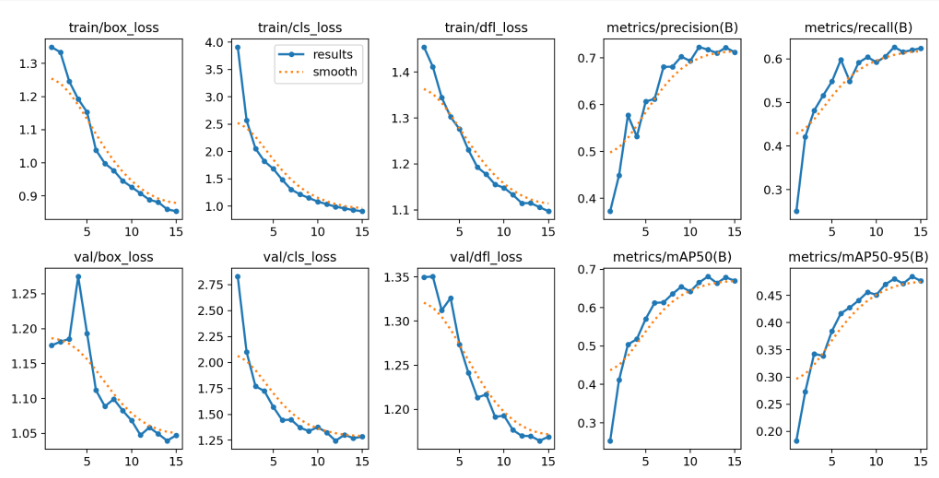
\includegraphics[width=0.5\textwidth]{4471_transfer_learning.png}
    \caption{Your caption here}
    \label{fig:yourlabel}
\end{figure}

\begin{figure}
    \centering
    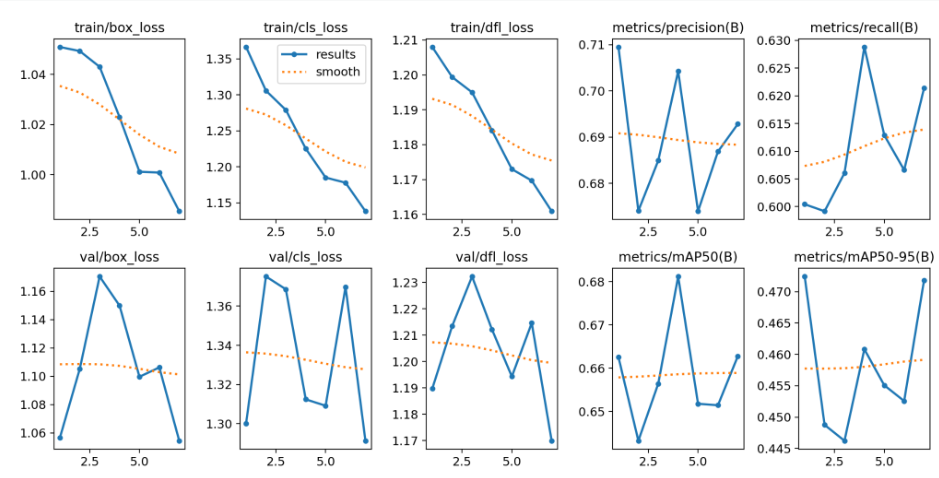
\includegraphics[width=0.5\textwidth]{4471_fine_tuning.png}
    \caption{Your caption here}
    \label{fig:yourlabel}
\end{figure}

\begin{figure}
    \centering
    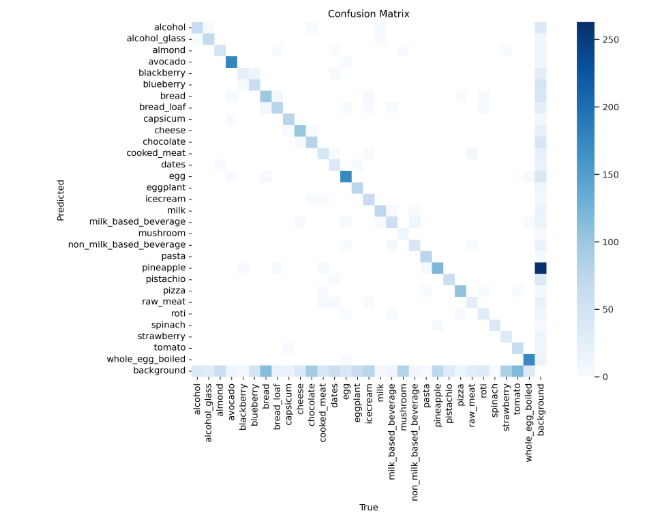
\includegraphics[width=0.5\textwidth]{4471_transfer_confusion.png}
    \caption{Your caption here}
    \label{fig:yourlabel}
\end{figure}

\begin{figure}
    \centering
    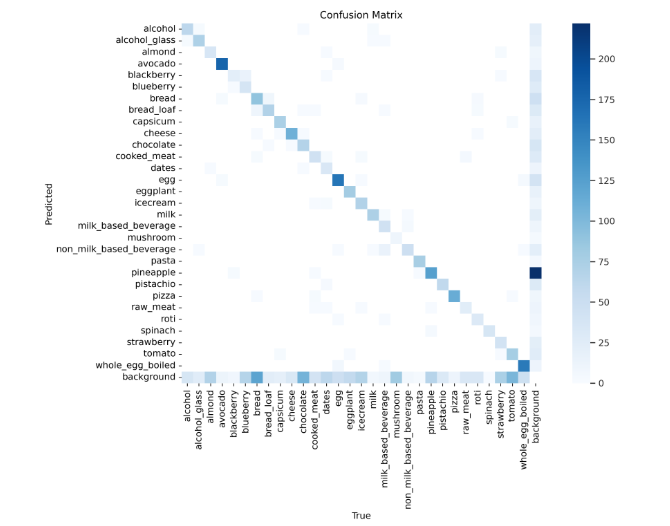
\includegraphics[width=0.5\textwidth]{4471_finetuning_confusion.png}
    \caption{Your caption here}
    \label{fig:yourlabel}
\end{figure}

%-------------------------------------------------------------------------
\section{Conclusion}
Required: Summarize your key results - what have you learned? 
Suggest ideas for future extensions or new applications of your ideas.

%-------------------------------------------------------------------------
\section{Supplementary Material}
Required: not counted toward your 6-8 page limit and submitted as a separate file. Your supplementary material might include:
Source code (if your project proposed an algorithm, or code that is relevant and important for your project.).
Cool videos, interactive visualizations, demos, etc.

%%%%%%%%% REFERENCES
{
    \small
    \bibliographystyle{bibliostyle}
    \bibliography{bibliography}
}

\end{document}
